% -*- root: ../thesis.tex -*-
%!TEX root = ../thesis.tex

% ******************************* Thesis Chapter 1 ****************************

% the code below specifies where the figures are stored
\ifpdf
    \graphicspath{{chapters/1_introduction/figures/}}
\else
    \graphicspath{{1_introduction/figures/EPS/}{1_introduction/figures/}}
\fi
% ----------------------------------------------------------------------
%: ----------------------- introduction content ----------------------- 
% ----------------------------------------------------------------------


\ac{ML} has become a wide field of research with a variety of subfields, each dedicated to solve various problems in different ways.
\textit{Probabilistic machine learning}, in particular, aims at representing the different models, using paradigms and tools from statistics.

\begin{itemize}
    \item Motivate the idea of Bayesian machine learning
    \item Bring to the concept of relation between representation and inference
    \item Introduce each of the chapter properly
\end{itemize}


\section{Bayesian Machine Learning}

\begin{itemize}
    \item Bayes is awesome
    \item Frequentist vs Bayesian
\end{itemize}

Some problems in \ac{ML} have critical requirements, such as probability guarantees for the predictions or working with meaningful interpretable models.
The Bayesian framework brings both by inferring probability distributions instead of point estimates.
For a given model, by setting a prior distribution over the parameters, the \textit{posterior} represent the updated belief we have about our model after observing some data.
This allows to model uncertainty in a principled way and to prevent overfitting in the low-data regime.
However, they come at a higher computational cost: a distribution contains more information than a single point, finding analytical solutions is rare and often require involved manual derivations.

% Bayesian Machine Learning is just another name for applied statistics on clean datasets.
A typical example is in medicine, where data is scarce, but the predictive outcome can have a dramatic effect (diagnosis, prognosis, etc...).



\section{The underestimated power of choosing representations}

\begin{itemize}
    \item Different representation lead to very different results, efficiency etc.
    \item Mention existing approaches
\end{itemize}
The leading thread of this thesis is \textit{representations} and how to use them to solve problem more efficiently with less work.
When modelling statistical problems, one needs to define relations between variables (observed and latent) and choose appropriate distributions to represent those.
Some modelling choices are equivalent conceptually but have drastic differences when it comes to inference.
A neat example, presented in \citet{gorinovaAutomaticReparameterisationProbabilistic2020}, is the so-called Neal's funnel.
There are two equivalent representations, called centered and non-centered, where one leads to an inference nightmare while the other is a nice and easy isotropic Gaussian distribution.

\begin{minipage}{0.5\textwidth}
    \centering
    \begin{align}
        \begin{aligned}
            z \sim&\; \mathcal{N}(0, 3)\\
            x \sim&\; \mathcal{N}(0, \exp(z/2))
        \end{aligned}
    \end{align}
    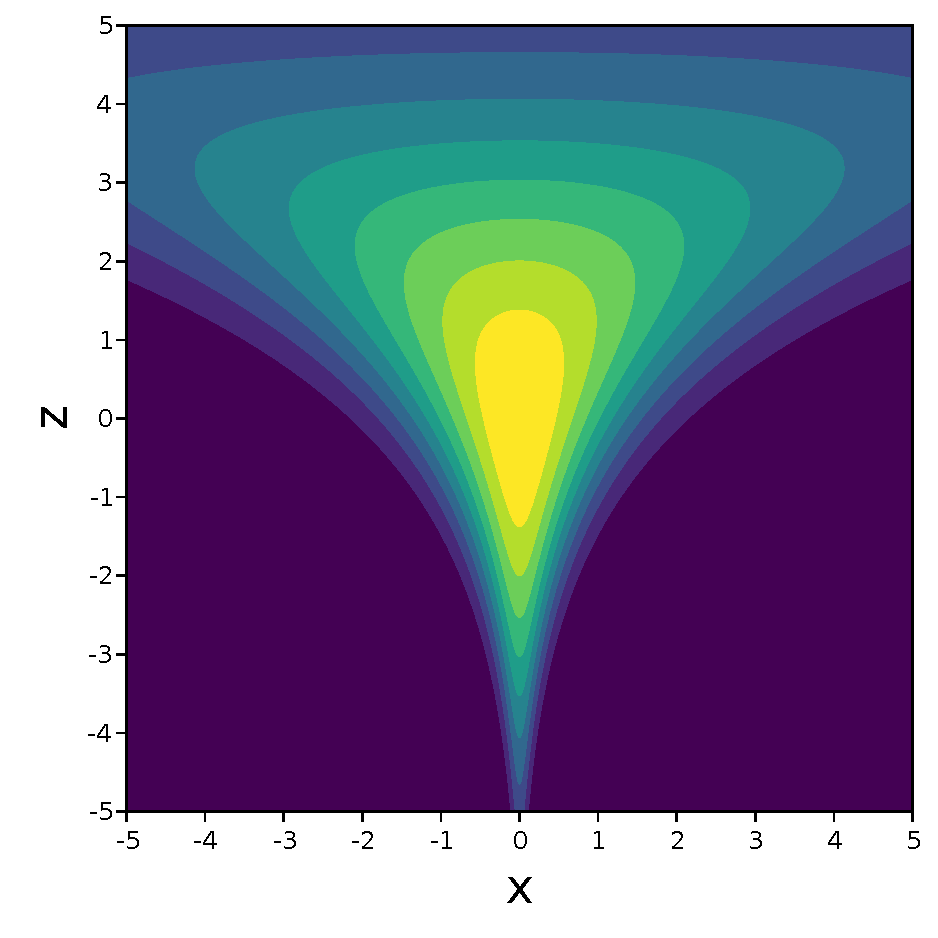
\includegraphics[width=\textwidth]{./chapters/1_introduction/figures/neals_funnel_centered.pdf}
    \captionof{figure}{Neal's funnel - Centered representation}
    \label{fig:neals_centered}
\end{minipage}
\begin{minipage}{0.5\textwidth}
    \centering
    \begin{align}
        \begin{aligned}
            \tilde{z} \sim&\; \mathcal{N}(0, 1),\quad z = 3\tilde{z}\\
            \tilde{x} \sim&\; \mathcal{N}(0, 1),\quad x = \exp(z/2)\tilde{x}
        \end{aligned}
    \end{align}
    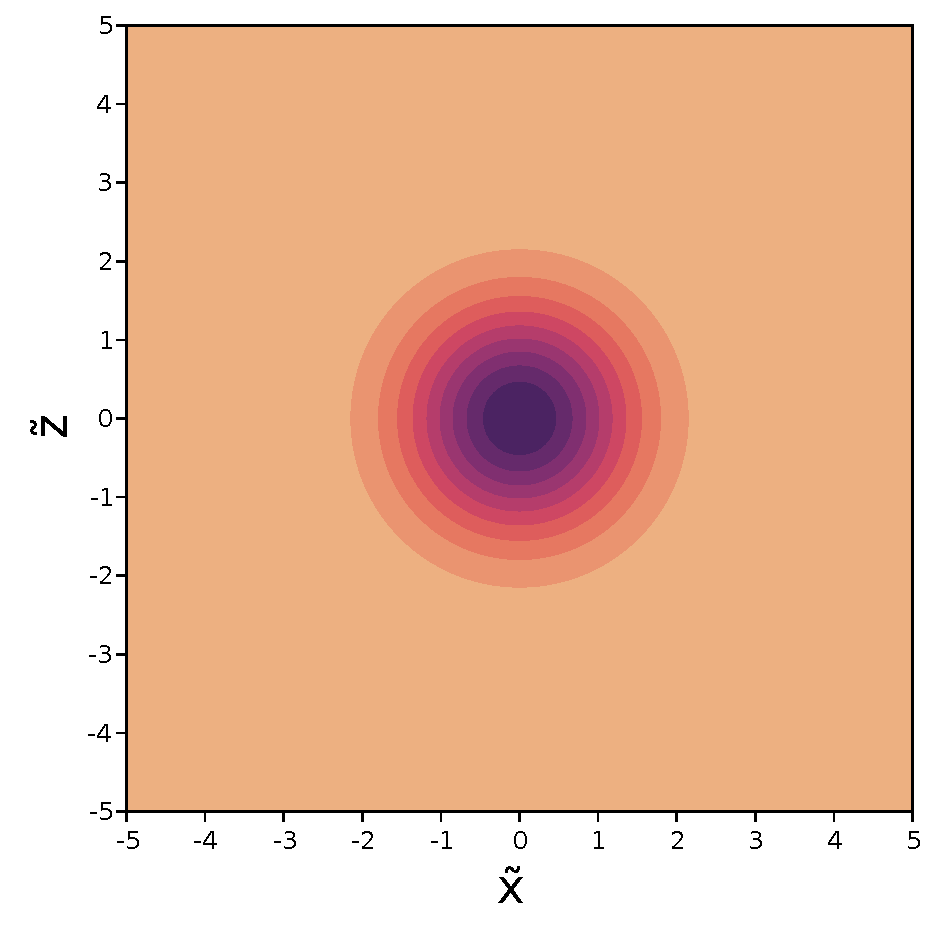
\includegraphics[width=\textwidth]{./chapters/1_introduction/figures/neals_funnel_non_centered.pdf}
    \captionof{figure}{Neal's funnel - Non-centered representation}
    \label{fig:neals_centered}
\end{minipage}
\vspace{0.5cm}

While both parametrization are one and the same, working with $p(\tilde{x},\tilde{z})$ is obviously simpler.
It is the same idea as working with spherical coordinates instead of Euclidean ones for electrodynamics. 

In this thesis, the various works presented focus on finding such representations where inference is made a lot easier and usually faster.
In particular, I will focus on the case where variables can be represented as (hierarchical) mixtures.
Defined later in Section \ref{sec:scale-mixtures}, variables that can be rewritten as scale-mixtures have a lot of advantages.
By writing them explicitly as mixtures, i.e. by adding more latent variables, inference can be made much easier while still being exact.
It brings the counter-intuitive view that adding more variables actually \textit{simplifies} the problem.


\section{Gaussian Processes}

\begin{itemize}
    \item All these things you can do with Gaussian processes
    \item why \ac{GPs} vs other things
\end{itemize}

Another large focus of this thesis are Gaussian based models and more particularly \acf{GPs}.
\ac{GPs} are strong tools to approximate functions using probabilistic methods.
Although they used to be reserved to regression problems, like the original \textit{krigging problem} \needcite, they can be used to represent any kind of function in a non-parametric way.
Compared to other general function approximators like neural networks, they have the advantage to directly contain information about the prediction's uncertainty.
Their non-parametric nature also allows avoiding overparametrization, while modern neural networks have billions of parameters to optimize, \ac{GPs} only depend on a mean function and a kernel function.
The Gaussianity of \ac{GPs} makes them the best candidate for the presented work on augmentation.
The focus on the likelihood augmentations has been aiming at making augmented likelihoods conditionally conjugate with Gaussian priors.


\section{Thesis Outline}

This thesis is constructed as follows:
\begin{itemize}
    \item Chapter \ref{ch:chapter2} will introduce in details all the common concepts to Bayesian inference and \ac{GPs}.
          This background is generally introduced in each of the published articles, but this chapter allows going more in-depth in the background theory.
          Bayesian inference will be properly introduced with a focus on variational inference and sampling.
    \item Chapter \ref{ch:chapter3} introduces the paper \textit{Efficient Gaussian Process Classification Using P\`olya-Gamma Data Augmentation}, which was the first step of this thesis using augmentations to improve and scale up inference.
    \item Chapter \ref{ch:chapter4} introduced the paper \textit{Multi-Class Gaussian Process Classification Made Conjugate: Efficient Inference via Data Augmentation}.
          This paper brings new concepts of augmentation to a much more complex problem: multi-class classification.
    \item Chapter \ref{ch:chapter5} introduces the paper \textit{Automated Augmented Conjugate Inference for Non-conjugate Gaussian Process Models}.
          This work was the first generalization of one type of augmentation and allowed to get a much better understanding of these concepts.
    \item Chapter \ref{ch:chapter6} introduces the paper \textit{Flexible and Efficient Inference with Particles for the Variational Gaussian Approximation } a completely different way of performing variational inference with Gaussian distribution by using a continuous flows and particles.

\end{itemize}

